\pdfinfoomitdate=1
\pdftrailerid{}
\documentclass[12pt,letterpaper]{article}
\usepackage[margin=0.67in,headheight=16pt,headsep=20pt,footskip=26pt]{geometry}
\usepackage[T1]{fontenc}
\usepackage{lmodern}
\usepackage{tikz}
\usetikzlibrary{arrows.meta}
\usepackage{fancyhdr}
\usepackage{array}
\pagestyle{fancy}\fancyhf{}
\fancyhead[L]{\small Week 97 / Square remainders / Grades 3--5}
\fancyfoot[L]{\footnotesize Bellingham Math Circle / Week 97 / W97-35-v2}
\fancyfoot[R]{\footnotesize\thepage}
\renewcommand{\headrulewidth}{0.4pt}\renewcommand{\footrulewidth}{0pt}
\setlength{\parindent}{0pt}\setlength{\parskip}{9pt}
\renewcommand{\familydefault}{\sfdefault}
\newcommand{\problem}[2]{\textbf{Problem #1:} #2\par}
\newcommand{\blank}[1]{\begin{tikzpicture}\draw[gray!45,rounded corners=3pt] (0,0) rectangle (17.9,#1);\end{tikzpicture}}
\newcommand{\dotat}[2]{\fill[black!75] ({#1},{#2}) circle(0.085);}
\newcommand{\support}[2]{\begin{tikzpicture}\draw[gray!55,rounded corners=3pt] (0,0) rectangle(3.35,0.85);\node at(1.675,0.425){\small $#1\times #1=#2$};\end{tikzpicture}}
\begin{document}
\fontsize{13}{17}\selectfont

An input of 3 means a $3\times3$ square of counters. Input 0 uses no counters. Remove complete bundles of the given size until fewer than one bundle's worth remain. The number left is the output; it can be 0.

\begin{center}
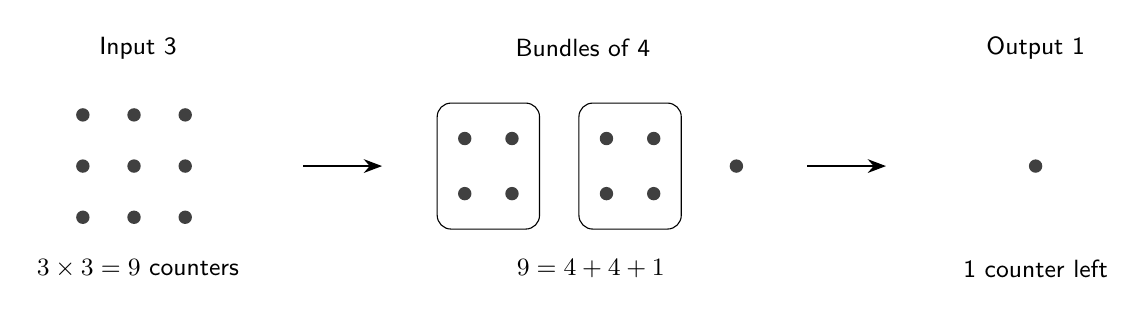
\begin{tikzpicture}[x=1cm,y=1cm,>=Stealth]
\node at(1.6,2.8){\small Input 3};
\foreach \x in {0,1,2} \foreach \y in {0,1,2} {\dotat{0.9+0.65*\x}{0.65+0.65*\y}}
\node at(1.6,0){\small $3\times3=9$ counters};
\draw[->,thick] (3.7,1.3)--(4.7,1.3);
\node at(7.25,2.8){\small Bundles of 4};
\foreach \a in {5.4,7.2} {
\draw[rounded corners=5pt] (\a,0.5) rectangle +(1.3,1.6);
\foreach \x in {0,1} \foreach \y in {0,1} {\dotat{\a+0.35+0.6*\x}{0.95+0.7*\y}}}
\dotat{9.2}{1.3}
\node at(7.35,0){\small $9=4+4+1$};
\draw[->,thick] (10.1,1.3)--(11.1,1.3);
\node at(13,2.8){\small Output 1};
\dotat{13}{1.3}
\node at(13,0){\small 1 counter left};
\end{tikzpicture}
\end{center}

With bundles of 4 and only inputs 0--3:
\begin{center}
\setlength{\tabcolsep}{15pt}
\begin{tabular}{r|cccc}
Input & 0 & 1 & 2 & 3\\
Output & 0 & 1 & 0 & 1
\end{tabular}
\end{center}
Output 1 hides two possible inputs: 1 and 3. There are two different outputs: 0 and 1.

\problem{1}{Build squares with inputs 0, 1, 2, 3 and 4. Use bundles of 5. Find every pair of different inputs that leaves the same output. Which outputs from 0 to 4 cannot occur?}

\begin{center}
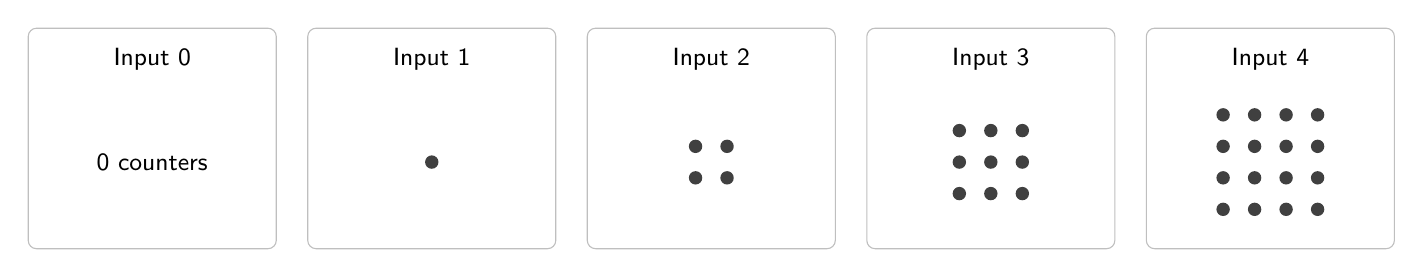
\begin{tikzpicture}[x=1cm,y=1cm]
\foreach \n in {0,1,2,3,4}{
\pgfmathsetmacro{\left}{3.55*\n}
\draw[gray!50,rounded corners=3pt] (\left,0) rectangle +(3.15,2.8);
\node at(\left+1.575,2.4){\small Input \n};
\ifnum\n=0 \node at(\left+1.575,1.1){\small 0 counters};\else
\foreach \x in {1,...,\n}\foreach \y in {1,...,\n}{\dotat{\left+1.575+(\x-(\n+1)/2)*0.4}{1.1+(\y-(\n+1)/2)*0.4}}\fi
}
\end{tikzpicture}
\end{center}
\blank{6.0}

\newpage

\problem{2}{Use bundles of 7 and inputs from 0 to 6. Choose a secret input, make its square, and tell your partner only the output. Your partner must name every possible input. Switch roles. Among outputs that occur, find those that hide the most possible inputs and the fewest possible inputs.}

\begin{center}
\support{0}{0}\quad\support{1}{1}\quad\support{2}{4}\\[8pt]
\support{3}{9}\quad\support{4}{16}\quad\support{5}{25}\\[8pt]
\support{6}{36}
\end{center}
\blank{13.6}

\newpage

\problem{3}{Use bundles of 7, 8 and 9, each with inputs from 0 to one less than the bundle size. For each bundle size, find all outputs that hide the most possible inputs. Which bundle size has an output that hides the most inputs?}

\begin{center}
\support{0}{0}\quad\support{1}{1}\quad\support{2}{4}\\[8pt]
\support{3}{9}\quad\support{4}{16}\quad\support{5}{25}\\[8pt]
\support{6}{36}\quad\support{7}{49}\quad\support{8}{64}
\end{center}
\blank{13.6}

\newpage

\problem{4}{A secret input is one of the whole numbers 0--14. Its square leaves output 1 after removing bundles of 15. Find every possible input. Could a different output hide even more inputs?}

\begin{center}
\support{0}{0}\quad\support{1}{1}\quad\support{2}{4}\\[8pt]
\support{3}{9}\quad\support{4}{16}\quad\support{5}{25}\\[8pt]
\support{6}{36}\quad\support{7}{49}\quad\support{8}{64}\\[8pt]
\support{9}{81}\quad\support{10}{100}\quad\support{11}{121}\\[8pt]
\support{12}{144}\quad\support{13}{169}\quad\support{14}{196}
\end{center}
\blank{11.1}

\newpage

\problem{5}{Use bundles of 7. Could an input bigger than 6 produce an output that none of the inputs 0--6 produced? Settle the question for every whole-number input. Give an explanation that also works for squares too big to build.}

\begin{center}
\support{7}{49}\quad\support{8}{64}\quad\support{9}{81}\\[8pt]
\support{10}{100}\quad\support{11}{121}\quad\support{12}{144}\\[8pt]
\support{13}{169}\quad\support{14}{196}\quad\support{15}{225}
\end{center}
\blank{14}

\newpage

\problem{6}{Compare bundle sizes 3, 5, 7 and 11. Each time, use inputs from 0 to one less than the bundle size. Find a rule connecting the bundle size to the number of different outputs that occur. Count output 0 too. These bundle sizes are odd primes: their only positive divisors are 1 and themselves. Can you explain why your rule works for every odd prime? Does it also work for 8, 9 or 15?}

\begin{center}
\support{0}{0}\quad\support{1}{1}\quad\support{2}{4}\\[8pt]
\support{3}{9}\quad\support{4}{16}\quad\support{5}{25}\\[8pt]
\support{6}{36}\quad\support{7}{49}\quad\support{8}{64}\\[8pt]
\support{9}{81}\quad\support{10}{100}
\end{center}
\blank{10.9}
\end{document}
